\documentclass{article}
%\usepackage{epsfig,graphicx,pstricks}
\usepackage{graphicx,pstricks}
\usepackage{listings}
\input /home/jaosborn/research/mymacs.tex
\oddsidemargin  0pt
\evensidemargin 0pt
\marginparwidth 1in
\marginparsep 0pt

\pagestyle{empty}

\topmargin 0pt
\headheight 0pt
\headsep 0pt
\topskip 0pt

\footskip 0pt
\textheight 9in
\textwidth 6.5in

\def\bfblue#1{{\bf {\blue #1}}}
\definecolor{lightgray}{rgb}{.7,.7,.7}
\newsavebox\lstbox
%                keywordstyle=\footnotesize\color{blue}\ttfamily,
\lstset{language=SAS, frame=tlrb, showspaces=FALSE,
                basicstyle=\footnotesize\ttfamily,
                keywordstyle=\footnotesize\ttfamily,
}
\lstdefinestyle{BashOutputStyle}{
  basicstyle=\small\ttfamily,
  numbers=none,
  frame=tblr,
  columns=fullflexible,
  backgroundcolor=\color{blue!10},
  linewidth=0.9\linewidth,
  xleftmargin=0.1\linewidth
}

\def\bfl{\begin{lstlisting}[basicstyle=\footnotesize\ttfamily, keywordstyle=\footnotesize\ttfamily,showspaces=FALSE,showstringspaces=FALSE]}
\def\bflf{\begin{lstlisting}[basicstyle=\footnotesize\ttfamily, keywordstyle=\footnotesize\ttfamily,frame=TRLB,showstringspaces=FALSE]}
\def\btl{\begin{lstlisting}[basicstyle=\tiny\ttfamily, keywordstyle=\tiny\ttfamily,showspaces=FALSE,showstringspaces=FALSE]}
\def\btlf{\begin{lstlisting}[basicstyle=\tiny\ttfamily, keywordstyle=\tiny\ttfamily,frame=TRLB,showstringspaces=FALSE]}













\begin{document}
\centerline{Modelling the distribution of aflatoxin amount by kernel}
\centerline{Analyzing Tom Whitaker's data}
\centerline{Jason Osborne, February, 2019}
%Here is an black space for an answer \rule{1.7in}{.2mm}
In each of 20 lots of almonds, there were 16 samples, each of 100g of crushed 
up almonds.  Each sample consisted of $N=7730$ almonds.  ({\em is this right?})
A measurement for sample $j$ from lot $i$, $\bar{X}_{ij}$ is obtained by 
dividing the observed ppb of aflatoxin, $X_{ij}$ by the number of kernels in the 
sample:   $\bar{X}_{ij}=(X_{ij}/N)$.  So, $X_{ij}$ is really a sum of $N$ kernels,
$$X_{ij}=\sum_{l=1}^N X_{ijl}.$$
%$X_{ij}$ is then the theoretical aflatoxin count for a kernel sampled 
%from lot $i$.  
This analysis aims to quantify the distribution of $X_{ijl}$ for a 
given lot, given observed summary statistics as described below.

The averages of the measured concentrations from the 16 samples from each 
lot $i$ are denoted 
$$\bar{X}_i=\frac{1}{16} \sum_1^{16}(X_{ij}/N) = \frac{1}{16} \sum_j \bar{X}_{ij} \ \ \ \ \ \mbox{ for } \ i=1,\ldots,20$$  
The sample
variance among the 16 aflatoxin concentration sample averages from lot $i$ is denoted $S_i^2$:
$$ S_i^2 = \frac{1}{16-1} \sum_{j=1}^{j=16} (\bar{X}_{ij}-\bar{X}_i)^2\ \ \ \ \ \mbox{ for } \ i=1,\ldots,20$$  


The negative binomial distribution %with parameters $M_i$ and $K_i$ is 
is proposed to model ppb among kernels.  The general form of this distribution, with mean parameter $M$ and shape parameter $K$, and its moments are given below.
Let $X_{ijl}$ denote the ppb of a kernel sampled from sample $j$, lot $i$ (even though sampling of individual kernels is not possible).  Then
%\begin{eqnarray*}
\[
\begin{array}{ccccc}
P(X_{ijl}=x) &=& \choose{x+K_i-1}{K_i-1}\left(\frac{K_i}{M_i+K_i}\right)^{K_i} \left(\frac{M_i}{M_i+K_i}\right)^x & \mbox{ for } & x=0,1,2,\ldots \\
E(X_{ijl}) &=& M_i & = & \mu\\
V(X_{ijl}) &=& M_i + M_i^2/K_i & = & \sigma^2
\end{array}
\]
%\end{eqnarray*}

If the distribution among kernels is negative binomial with parameters $M$ and $K$, then the sum of ppb in a sample ($j$) and lot ($i$)
is also negative binomial, under the simplifying assumptions that the kernels are a random sample from the lot.  The mean parameter is $NM_i$ and 
the shape parameter is $NK_i$.  The mean and variance
are given by
\begin{eqnarray*}
E(X_{ij}) &=& E(N\bar{X}_{ij}) = NM_i \\
V(X_{ij}) &=& V(N\bar{X}_{ij}) = NM_i + (NM_i)^2/(NK_i)
\end{eqnarray*}
For an average (or measurement on a sample $j$), $\bar{X}_{ij}=X_{ij}/N$, the moments are 
\begin{eqnarray*}
E(\bar{X}_{ij}) &=& M_i \\
V(\bar{X}_{ij}) &=& \frac{1}{N^2} (NM_i + (NM_i)^2/(NK_i)) \\
&=& \frac{M_i}{N} + M_i^2/(NK_i)
\end{eqnarray*}
For averages of sample averages, and sample variances like those appearing in the spreadsheet:
\begin{eqnarray*}
\bar{X}_{i} &=& \frac{1}{16} \sum_{j=1}^{16} \bar{X}_{ij} \\
E(\bar{X}_{i}) &=& E(\frac{1}{16} \sum_{j=1}^{16} \bar{X}_{ij}) = M_i \\
%V(\bar{X}_{i}) &=& \frac{1}{16} V(\bar{X}_{ij}) = \frac{1}{16}\left(\frac{M_i}{N} + M_i^2/K_i\right) \\
%E(V(\bar{X}_{i})) &=& ??
%E(S_i^2) &=& \left(\frac{M_i}{N} + M_i^2/K_i\right) 
E(S_i^2) &=& V(\bar{X}_{ij}) = \frac{M_i}{N} + M_i^2/(NK_i)
\end{eqnarray*}
\newpage
The {\em method of moments} sets the first two sample moments equal to their 
expectation, obtaining a system of two equations and two unknowns:
\begin{eqnarray*}
\bar{X}_i & \stackrel{\mbox{set}}{=} & M_i  \\
S^2_i & \stackrel{\mbox{set}}{=} & \left(\frac{M_i}{N} + M_i^2/(NK_i)\right)
\end{eqnarray*}
The solution $(\hat{M}_i,\hat{K}_i)$ is given by 
\begin{eqnarray*}
\widehat{M}_i &=& \bar{X}_i \\
\widehat{K}_i &=& \frac{\widehat{M_i}^2}{NS_i^2 - \widehat{M_i}}
\end{eqnarray*}
The estimated parameters for all 20 lots appear in the plots below, with shape parameters ($k$) on the vertical axis and lot mean on the horizontal axis.  The plot on the left allows for a non-zero intercept, the plot on the right is through the origin.  Both provide some indication of a positive association between estimated shape and scale.  Lots with more aflatoxin also tend to have 
a larger estimated shape parameter.  The lot with the largest shape parameter may be an outlier of sorts.
\begin{center}
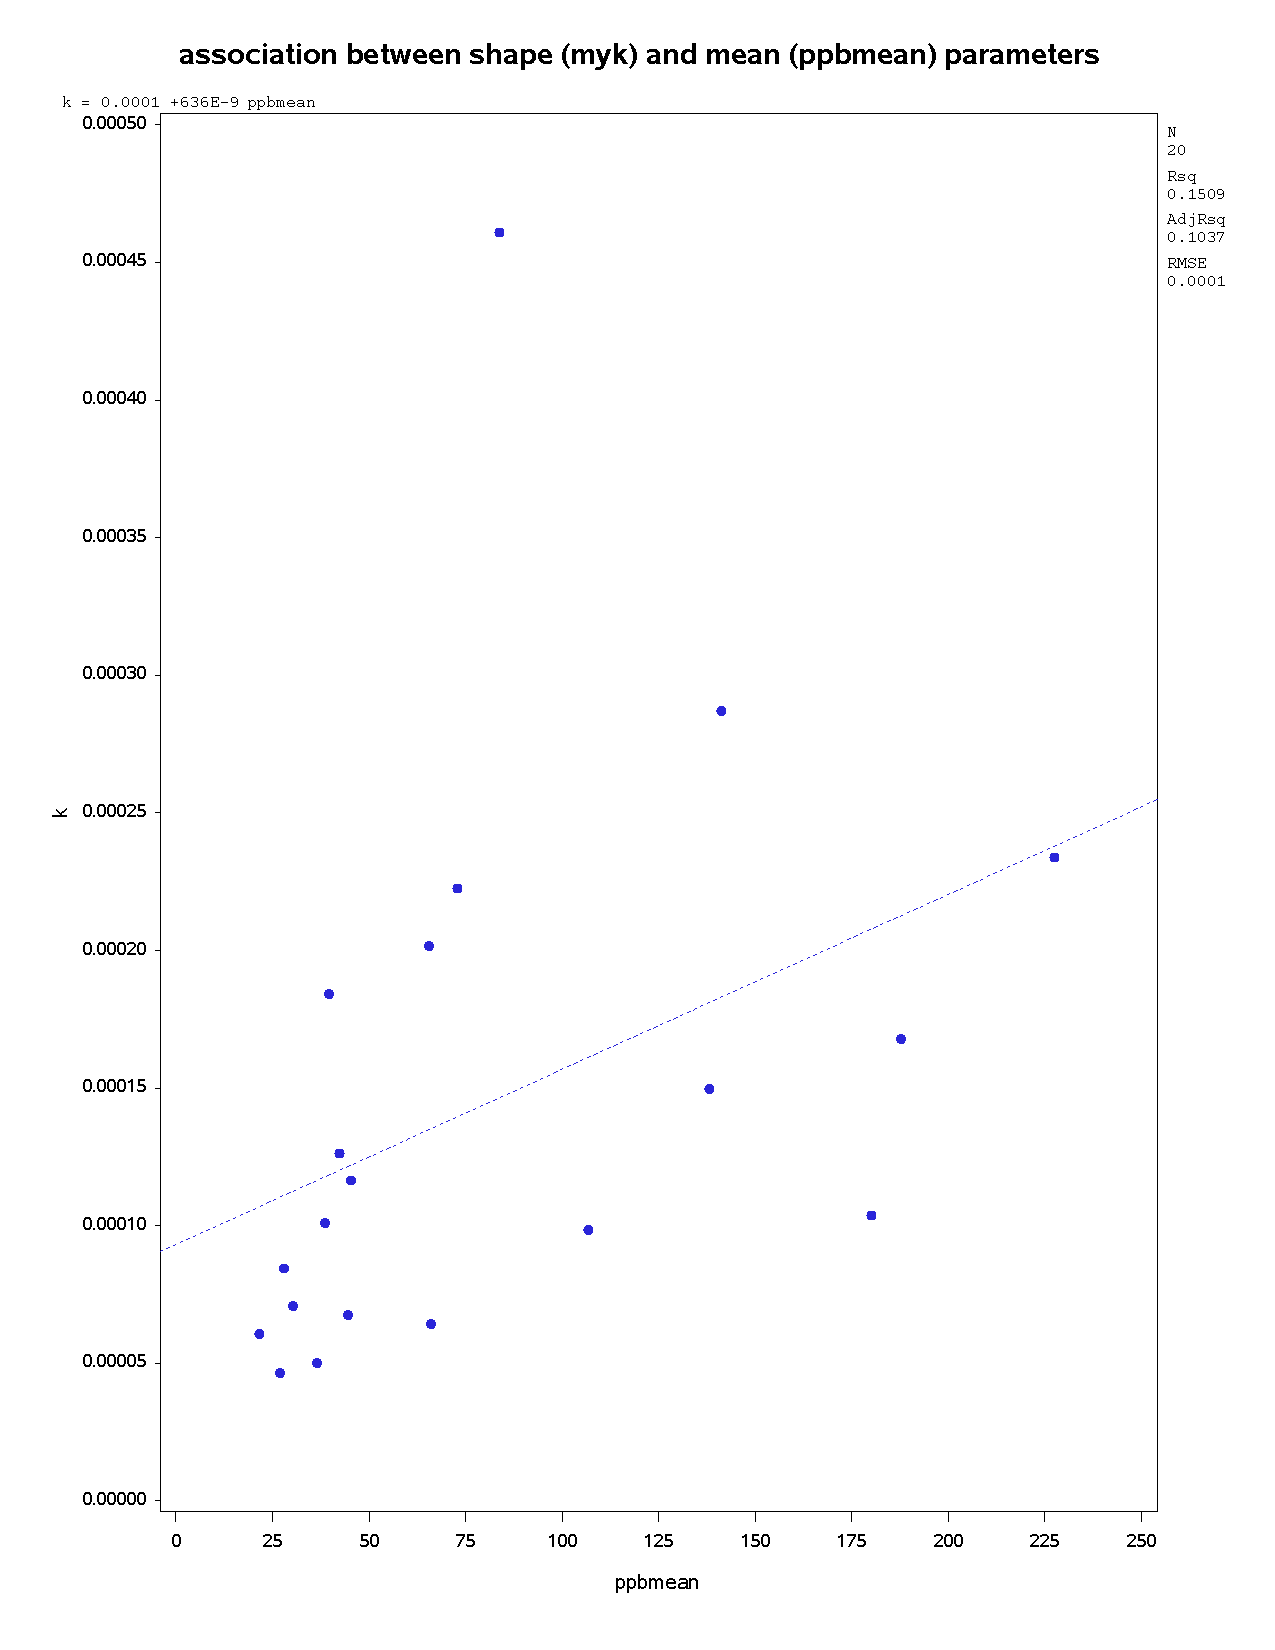
\includegraphics[scale=.35]{k_linear_M.pdf}
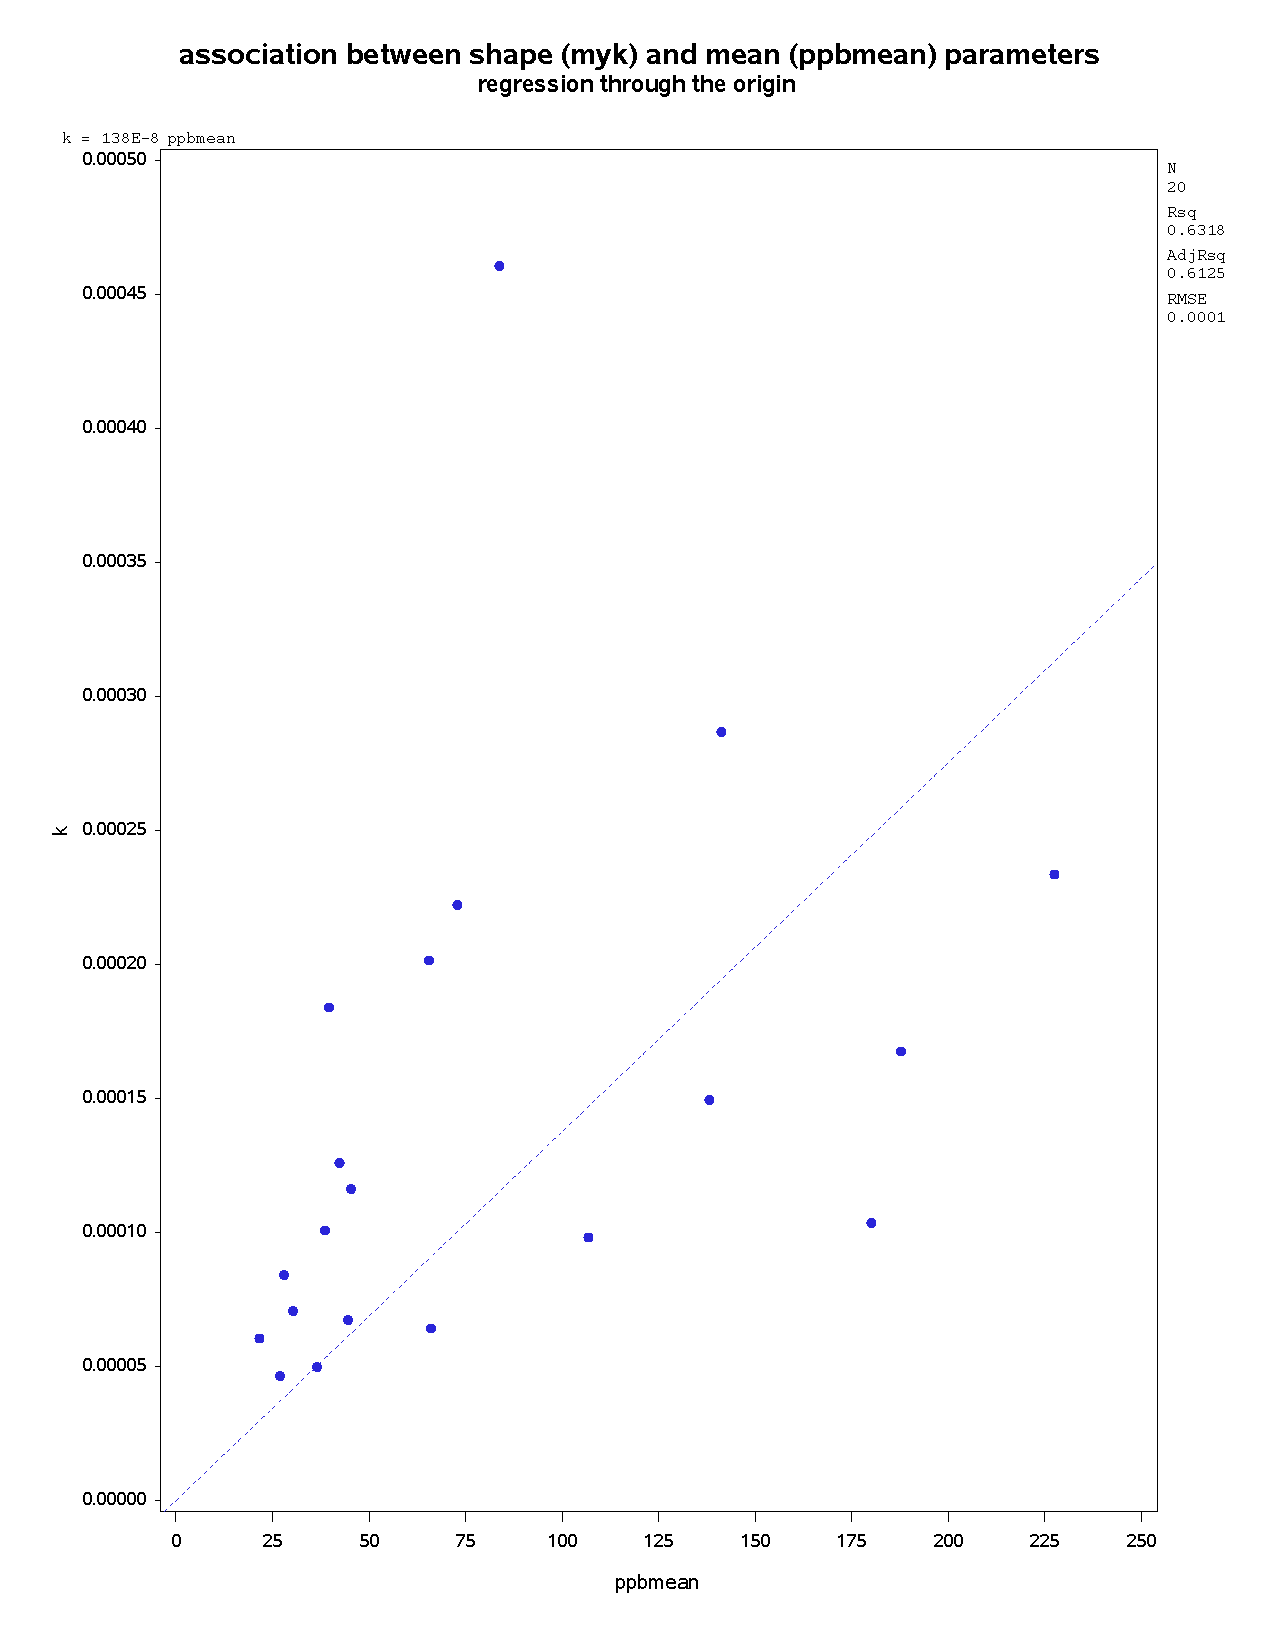
\includegraphics[scale=.35]{k_linear_M_origin.pdf}
\end{center}
\newpage
For each of the points (lots) in these plots, there were 16 samples, and from these samples, one 
or two subsamples were taken and from these subsamples, one or two aliquots were taken.  This 
nested measurement is useful for estimating sources of variation in the assessment of aflatoxin.
To assess the fit of the negative binomial model, the first aliquots from the first subsamples
from each sample of each lot were used in empirical distribution function (ECDF) plots.  The
ECDF for a given lot at any concentration is simply the proportion of samples from
that lot (out of 16) with an average that was less than or equal to the concentration.  This is naturally
a step-function with jump discontinuities at the observed concentration amounts for each sample.
At each such concentration, the function increases by $1/16$ since there are 16 sample averages
per lot.  
This function is a nonparametric and unbiased estimate of the real cumulative distribution function
for averages of $N$ kernels.  The distribution of aflatoxin in a sum of $N$ kernels from lot $i$, 
$X_{ij}=\sum_l X_{ijl}$ is also negative binomial, with mean $N M_i$ and $N K_i$.  This fact can be
used to obtain an expression for an estimate of the theoretical distribution function for the
averages from lot $i$.
Using the probability mass function for kernels, $X_{ijl}$ from
the previous page, we have
\begin{eqnarray*}
 P(\bar{X}_{ij} \leq x) &=& P(\sum_l X_{ijl} \leq N x) \\
  &=& P(X_{ij} \leq N x) \\
%&=& \sum_{t=0}^{[Nx]} P(X_{ij}=x;N\widehat{M}_i,N\widehat{K}_i) 
&=& \sum_{t=0}^{[Nx]} P(X_{ij}={\red t};N\widehat{M}_i,N\widehat{K}_i) 
\end{eqnarray*}
Here, $[Nx]$ is the largest integer less than or equal to $Nx$.
%Plots in which the estimated negative binomial cumulative distribution function are
%overlaid with the ECDF for the 20 lots are given below: \\
All statistical software packages have this function built-in.  In SAS, the generic {\tt CDF} function
may be used along with the 'NEGB' parameter:
\bfl
cdfhat = CDF('NEGB',N*xbar,phat,N*khat);
\end{lstlisting} 

%This function is an unbiased and nonparametric estimate of the real cumulative 
%distribution function for kernels, which can be estimated by substitution of the parameter 
%estimates $\widehat{M}_i$
%and $\widehat{K}_i$ into the cumulative distribution function that accumulates the probability
%masses given in the expression for $P(X_{ijl}=x)$ given on the prior page.  
%\begin{eqnarray*}
% P(X_{ijl} \leq x) &=& \sum_{t=0}^{[x]} P(X_{ijl}=x;\widehat{M}_i,\widehat{K}_i) \\
%&=& \sum_{t=0}^{[x]}\choose{t+\widehat{K_i}-1}{\widehat{K_i}-1}\left(\frac{\widehat{K_i}}{\widehat{M_i}+\widehat{K_i}}\right)^{\widehat{K_i}} \left(\frac{\widehat{M_i}}{\widehat{M_i}+\widehat{K_i}}\right)^t 
%\end{eqnarray*}
%Here, $[x]$ is the largest integer less than or equal to $x$.

Plots in which the estimated negative binomial cumulative distribution function are
overlaid with the ECDF for the 20 lots are given below: \\

\begin{center}
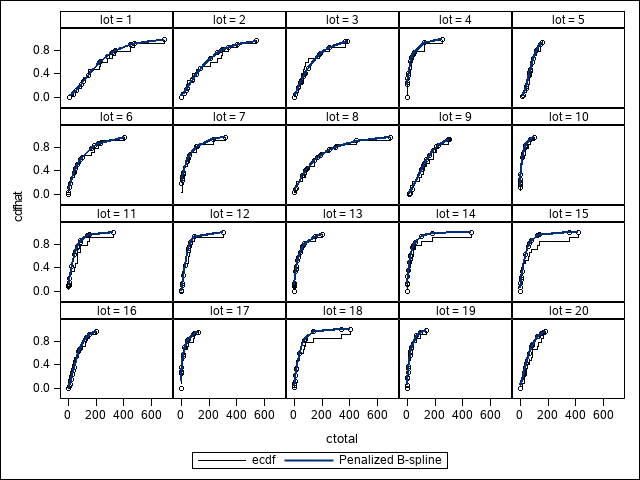
\includegraphics[scale=.7]{SGPanel5x4.png}
\end{center}

The step function makes no assumptions about the distribution of
aflatoxin among kernels, and the blue line is a smoothed version of the
function which assumes aflatoxin among kernels follows the negative binomial
distribution.  
There appears to be reasonable agreement between these two estimate of the
distribution functions associated with the sample averages of all $N=20$
lots.  
%
% added the following text March 4
%
{\blue
To formally assess the goodness-of-fit of the Negative Binomial model, one
could obtain the Kolmogorov-Smirnov test statistic, which is the maximum
distance between the estimate based on the Negative Binomial assumption and
the ECDF across all values of the aflatoxin sum for each lot.  To see
whether or not these differences exceed the $\alpha=.05$ level critical 
value, $D_{nn}$ for this test using $n=16$ samples per lot, the ECDF was 
plotted with limits of the form $\pm D_{nn}=.3273$.  In none of the lots
did the Negative Binomial estimate fall outside of this interval about
the ECDF.  That is, the observed differences between the two estimates
of the distribution function for aflatoxin were not significant at level
$\alpha=.05$.}
 
%The estimated parameters of the latter distribution, $\hat{M}$ and
%$\hat{K}$ are based on aflatoxin measurements made from repeated measures (multiple
%subsamples per sample, multiple aliquots per subsample).
%Lots 14, 15 and 18 may be characterized
%by underestimated aflatoxin levels in the right tail and perhaps bear further inspection.
\end{document}



posited for kernels in sample $j$, lot $i$, then the mean and variance 
of the sample means from such a sample are given by
\begin{eqnarray*}
E(\bar{X}_{ij}) &=& M_i/N \\
\mbox{Var}(\bar{X}_{ij}) &=& \frac{1}{N}(M_i + M_i^2/K_i)
\end{eqnarray*}



If the mean and variance of a measurement of a sample $j$ from lot $i$ are 
denoted $\mu_i$ and $\sigma_i^2$, then
\begin{eqnarray*}
E(\bar{X}_i) &=& \mu_i \\
E(S_i^2) &=& V(\bar{X}_i) \\
&=& \sigma_i^2/N \\
\end{eqnarray*}
If the negative binomial distribution with parameters $M_i$ and $K_i$ is 
posited for kernels in lot $i$, then the mean and variance are given by
\begin{eqnarray*}
E(X_i) &=& M_i \\
\mbox{Var}(X_i) &=& M_i + M_i^2/K_i
\end{eqnarray*}
The population mean and variance of such a negative binomial distribution
are given below:
\begin{eqnarray*}
E(Y_i) &=& M_i \\
V(Y_i) &=& M_i+M_i^2/K_i
\end{eqnarray*}
Since the expectations of the summary statistics are given by
\begin{eqnarray*}
E(\bar{X}_i) &=& M_i \\
E(S_i^2) &=& V(Y_1)/N = (1/N)(M_i + M_i^2/K_i),
\end{eqnarray*}
the method-of-moments estimators of the negative binomial parameters for lot $i$ 
are
\begin{eqnarray*}
\widehat{M}_i &=& \bar{X}_i \\
\widehat{K}_i &=& \frac{\bar{X}_i^2}{NS_i^2-M_i} \\
\end{eqnarray*}
Inspection of the lot mean and variance statistics indicates a clear positive
relationship.  Lots with higher concentration also have higher mean. 
\begin{center}
\includegraphics{varmeanplot.pdf}
\includegraphics{sdmeanplot.pdf}
\end{center}
%The expectation of the lot variance may be estimated by
%$$ \widehat{E(S_i^2)} = V(X_i) = \frac{1}{N}$$


\end{document}
